\chapter{Result and Discussion}
\section{Result}
The following are the findings or results obtained from the selected model:
\subsection{Time requirements}
Table below shows the different time requirements for our project:
\begin{table}[H]
    \begin{tabular}{|l|l|}
    \hline
    S.N                & Average Time Required \\ \hline
    Feature Extratoion & 0.8 second per Image            \\ \hline
    Model Training with 20,000 images  & 10 minutes            \\ \hline
    Testing            & 30 second             \\ \hline
    \end{tabular}
    \caption{Time Requirements}
    \end{table}
\subsection{ROC Curve}
\begin{figure}[H]
    \centering
    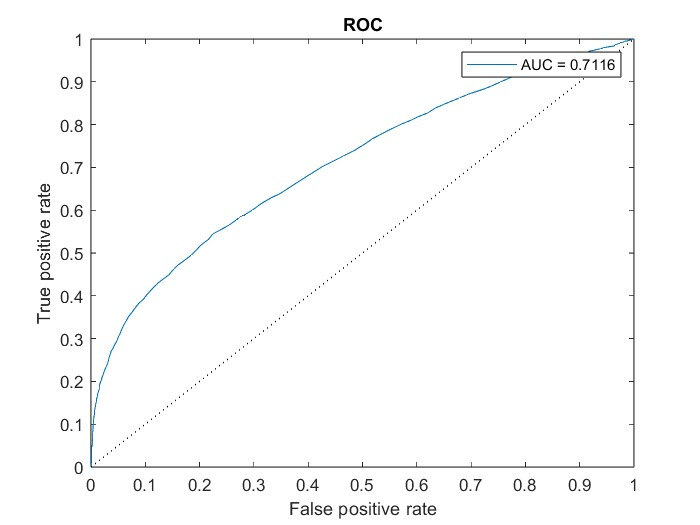
\includegraphics[width=120mm]{./img/2600/roc2600.jpg}
    \caption{ROC Curve}
\end{figure}
The ROC curve is a graphical representation of the contrast between true positive rates and the false positive rate at various thresholds. It is often used as a proxy for the trade-off between the sensitivity and the specificity of the model. The AUC is the area under the ROC curve. The higher the AUC, the better the performance of the model at distinguishing between the positive and negative classes.\\
We obtained Area Under the Curve (AUC) of 0.7116, indicating a high level of classification between positive and negative instances
\subsection{OOB Vs L}
\begin{figure}[H]
    \centering
    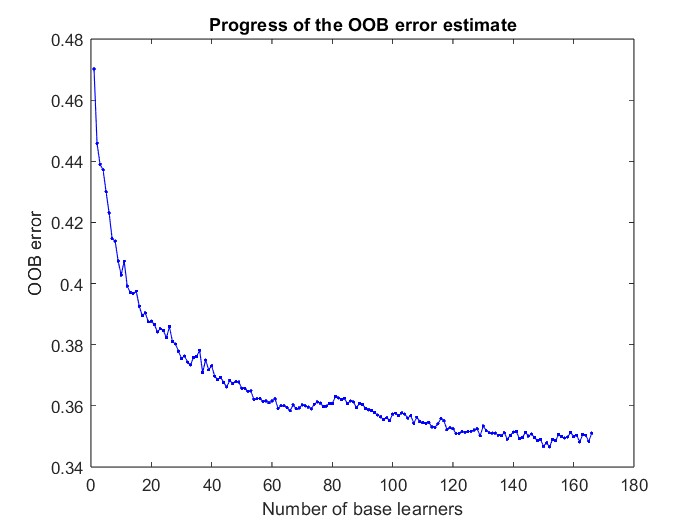
\includegraphics[width=120mm]{./img/2600/staturAATE2600.jpg}
    \caption{OOB Vs Number of Base Learners}
\end{figure}
Above graph shows different values of OOB error for different number of base learners. It is observed that the OOB error decreases as the number of base learners increases. The OOB error is minimum when the number of base learners is 160.
\subsection{Confusion Matrix}
\begin{table}[H]
\begin{figure}[H]
    \centering
    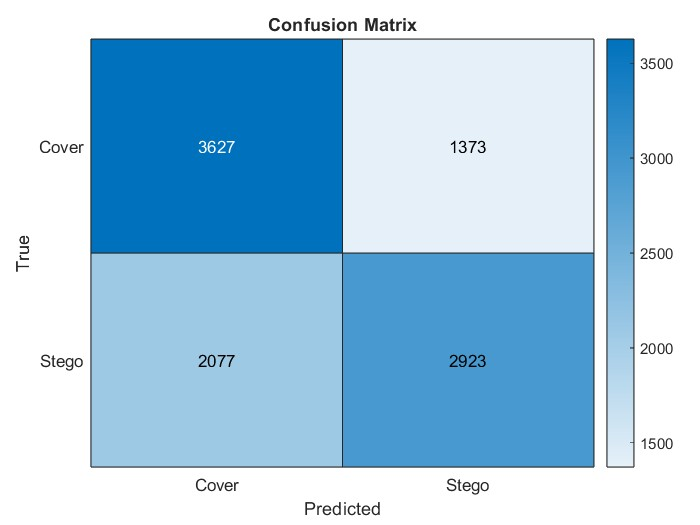
\includegraphics[width=120mm]{./img/2600/consuse2600.jpg}
\end{figure}
\caption{Confusion Matrix}
\end{table}
The model's classification performance is summarized through a confusion matrix, featuring 3627 true positives (correctly identified positives), 2923 false negatives (misclassified negatives), 2077 false positives (incorrectly labeled positives), and 1373 true negatives (correctly identified negatives). These metrics offer a concise yet comprehensive overview of the model's ability to distinguish between positive and negative cases, providing crucial insights for evaluating its effectiveness. The confusion matrix serves as a pivotal tool in assessing the model's strengths and weaknesses, contributing valuable information to the ongoing discourse on classification model refinement.
\subsection{Histogram}
\begin{figure}[H]
    \centering
    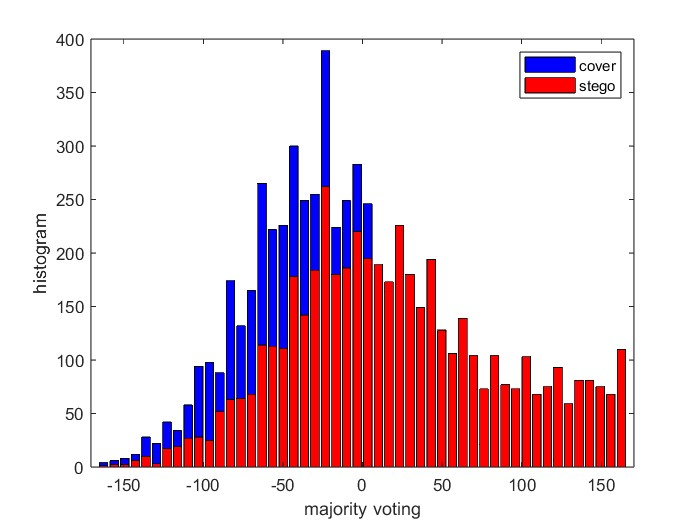
\includegraphics[width=120mm]{./img/2600/histo2600.jpg}
    \caption{Histogram of votes}
\end{figure}
The histogram of votes is a graphical representation of the number of votes for each class. The histogram provides a visual representation of the model's classification performance, offering insights into the distribution of votes across the different classes. The histogram is a valuable tool for evaluating the model's classification performance, providing a comprehensive overview of the distribution of votes and the model's ability to distinguish between positive and negative cases.

\section{Model Evaluation}
\subsection{Performance Metrices}
\subsection*{Precision}
Precision which is also called positive predictive value is the fraction of retrieved instances that are relevant. It is the ratio of true positive to the sum of true positive and false positive. It is given by the formula:
$$Precision = \frac{TP}{TP+FP} = \frac{3627}{3627+1373} = 0.73 $$
\subsection*{Accuracy}
Accuracy is the ratio of correctly predicted observation to the total observations. It is given by the formula:
$$Accuracy = \frac{TP+TN}{TP+TN+FP+FN}= \frac{3627+1373}{3627+1373+2077+2923}=0.65$$
\subsection{Recall}
Recall which is also called sensitivity is the fraction of relevant instances that have been retrieved over the total amount of relevant instances. It is the ratio of true positive to the sum of true positive and false negative. It is given by the formula:
$$Recall = \frac{TP}{TP+FN} = \frac{3627}{3627+2077}= 0.64$$






